

\section{DCNNFuzz Framework}
In this section, we first present an overview of the BLSTM-DCNNFuzz and then describe the main aspects in detail.  As seen in Fig. \ref{FigFramework}, the overall fuzzing framework includes Data Preprocessing Module(DPM), Model Training and MSG(message) Generating Module(MTMGM), MSG Sending and Receiving Module(MSRM) and Logging Module(LM). These modules collaborate with each other in completing fuzzing test tasks.



\subsection{Framework Overview}
The purpose of this framework is to conquer the aforementioned limitations of traditional fuzz testing methods. We make it meet these requirements: (i) Highly intelligent. It can design and generate test cases by itself. (ii) Protocol independence. It can deal with most ICPs without knowing their protocol specifications. (iii) Very efficient. The entire testing can be completed in just a few days. As for the general process, first, the framework fetches network traffic data from the target ICS. Then, it learns from the traffic data and generates various testing data. Finally, the data is injected into the target system for testing. The following describes the main steps.

\subsubsection{Preprocessing of ICP Communication Data}
Data preprocessing has a significant impact on model training. We take two steps to process the raw data. First, we cluster the raw data according to specific criteria. Then, we augment the test cases with a small percentage to increase their influence on forming the model. Lastly, we encode the raw data into a fully digital matrix form.

\subsubsection{Model Architecture and Training Strategies}
We use DCGAN as the underlying architecture. Our purpose is to generate aggressive fuzz testing data to attack the target ICP for triggering more bugs. To achieve this purpose, we carefully design the network structure of the generator and the discriminator. As to the model training, we take measures to handle the unstable training problem such as mode collapse and non-convergence. Lastly, we use the trained model to generate enough fuzzing data.

\subsubsection{Fuzz Testing The Target ICP}
In this step, we use the generated fuzzing data to attack a specific ICP. In the testing, we deliberately collect test cases that caused exceptions. They can enrich the original training data and help improve model performance. The following gives more detailed information about these steps.

\subsection{Preprocessing of ICP Communication Data}   %% %^^^^^^^^^^^^^^^^^
The current mainstream ICPs include Modbus, EtherCAT, Powerlink, Porfinet, Ethernet/IP, TSN (Time Sensitive Networks) [16], and so on. There are various ways to capture data packets from different ICPs. The most direct way is to use the appropriate terminal capture tool from the real industrial control network environment to capture the data packets generated by the ICSs as training data. After obtaining the raw data, Data Preprocessing Module (\textbf{DPM}) is divided into three steps to preprocess data. The details are as follows:

\subsubsection{Data Frame Clustering}
The effect of fuzz testing depends predominantly on the testing depth and high code coverage. Protocol messages captured from the ICP vary in length and message type. The better our model comprehends the differences between protocol messages, the better testing depth we can achieve. We leverage a variety of clustering strategies to improve the classification scores, such as frame length clustering, K-means clustering and so on. Frame length clustering is to cluster the sequences based on their length. Since sequences which have the same length always tend to share the same message type. K-means, using Euclidean distance as a similarity benchmark, is also applied in the clustering of data frames based on the function code of data frames. Under these strategies, we can do data augmentation to a class of messages with a small percentage. This makes the generated data more diverse, which can help improve code coverage.

\subsubsection{Adding Special Symbols}
The other step is to add special symbols to guide DPM to obtain higher quality training data. The process of capturing data by DPM can be divided into two categories, as shown in Fig. \ref{FigAddSpecialSymbols}. First, for a known protocol stack, such as the TCP/IP protocol stack which Modbus-TCP is running on, the IP header can be used as a demarcation point for capturing. We truncate the IP header (Including IP source address, destination address and additional information for some other delivery requests) and retain the file that holds the IP header for a further packet injection attack.  Then we insert STA (start) as the sequences start flag at the beginning of the packet body, END (end) as the sequences end flag. The operation eliminates the influence of irrelevant information on the model and improves the quality of the captured data. Second, if the protocol is unknown, the learning with the address is performed, and STA and END are added directly at the beginning and end of the entire captured data. Finally, the processed data is stored in the training data set.

Moreover, pad the short sequence with uniform character PAD(pad) to the maximum frame length. It helps unify the sequence length to standardize the training.
\begin{figure}[htbp]
	\centering
	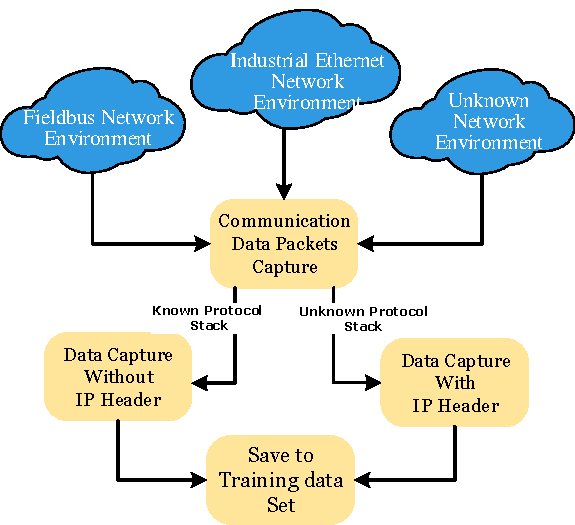
\includegraphics[width=3.2in]{FIGURE_LV/FigAddSpecialSymbols.pdf}
	\caption{Process of capturing data}
	\label{FigAddSpecialSymbols}
\end{figure}

\subsubsection{Data Feature Conversion}
The captured sequence data is in the native features which cannot be processed directly. In order for the model to perceive these features, raw digital protocol messages need to be converted to an appropriate pattern. Due to few ways to learn word embeddings \cite{levy2014neural} about data frames, we transfer the network traffic in the ICS into a hexadecimal sequence based on an alphabet of n characters.

In addition to the sequence length alignment, we use a character level preprocessing, inspired by \cite{zhang2015character}, to deal with the converted data feature in this work. In the alphabet of data frames, there are 10 digit characters and 6 English letter characters, as shown in the following:
\begin{figure}[htbp]   %  插入一栏图片
	\centering 
	
\includegraphics[width=2.2in]{FIGURE_LV/FIGURE_SET.pdf}
	%\caption{The alphabet}
	\label{FIGURE_SET}
\end{figure}

According to the alphabet, each character in the sequence is encoded as a one-hot vector of the $n$ dimension $x\in R^{1 \times n}$. As depicted in Fig. \ref{FigOneHot}, the position where the character locates in the alphabet is one, and the rest are zeros. Thus, a sequence data with length $l_0$ is encoded into a matrix $ X \in R^{l_0 \times n}$, as a stack of character embedding. 
\begin{figure}[htbp]
\centering
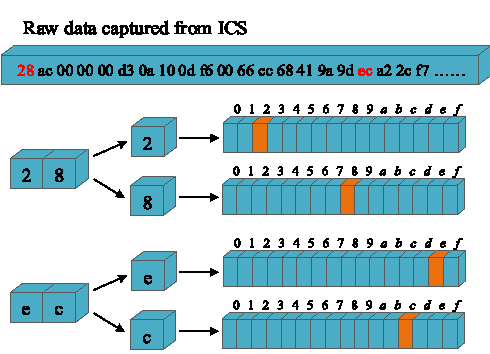
\includegraphics[width=3.2in]{FIGURE_LV/FigOneHot.pdf}
\caption{A sample of raw ICS data and its feature quantization}
\label{FigOneHot}
\end{figure}


\begin{figure*}[htbp] 		 %  插入双栏图片
	\centering
	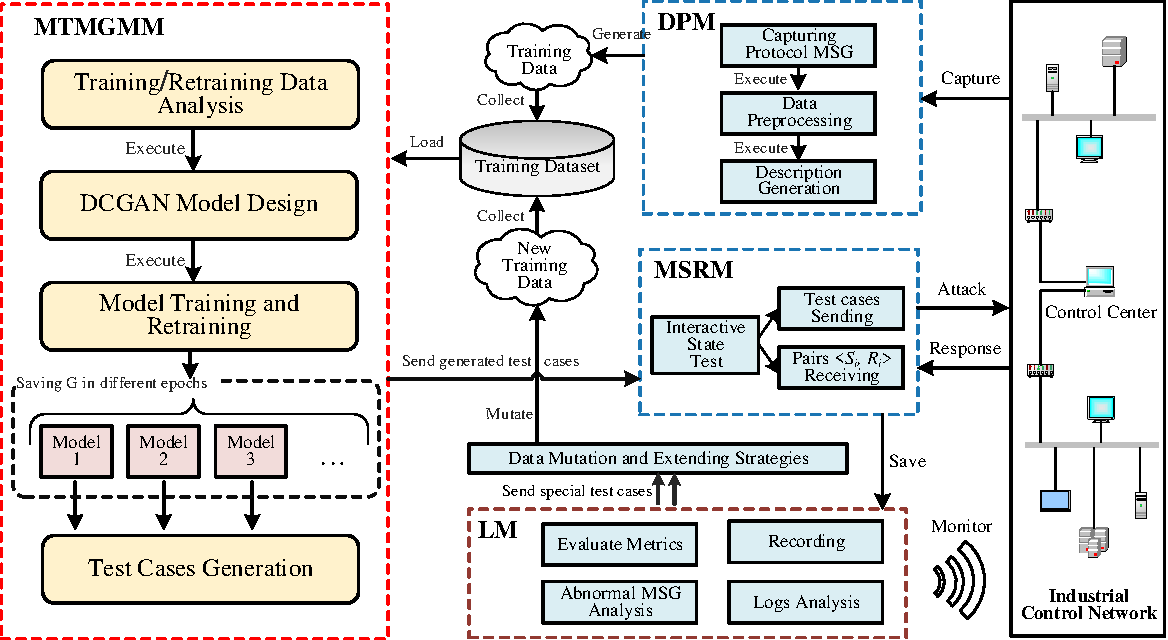
\includegraphics[width=5.5in]{FIGURE_LV/FigFramework.pdf}
	\caption{BLSTM-DCNNFuzz Framework}
	\label{FigFramework}
\end{figure*} 

\subsection{Model Architecture and Training Strategies}
In this section, we give the model architecture details of Model Training and MSG(message) Generating Module (\textbf{MTMGM}) as illustrated in Fig. \ref{FigModelArchitecture}. Later, we present the training strategies about the model in this study.

\subsubsection{Model Architecture}
There are two components, namely the generator model and the discriminator model. One of our design philosophies is to design lightweight models based on attaining its effect.  In virtue of the distinguishing feature of reducing the consumption of computing resources, it is convenient to deploy to embedded devices and lays the groundwork for continuous online learning in the future. Referring to the aforementioned DCGAN architecture constraints and our requirements, we reasonably designed the architecture of DCGAN which are given in Fig. \ref{FigModelArchitecture} (b). In general, the adversarial relationship between the $G$ and the $D$ can be expressed as follows:
\begin{equation}
\begin{array}{c}
{\min _G}{\max _D}V(D,G) = {E_{x\sim{P_x}}}\left[ {\log (D(x))} \right]\\
+ {E_{z\sim{P_z}}}\left[ { - \log (D(G(z)))} \right]
\end{array}
\end{equation}
where $D(x)$ indicates that the probability of $x$ is real, and $G(z)$ indicates that the probability distribution  of the sample data $z$. 

\quad \textit{\textbf{a. Generator.}} The generator uses a deconvolution \cite{dumoulin2016guide} neural network architecture. We adopt batch normalization (BN) right after each convolution and before activation, following \cite{ioffe2015batch}. In addition, The generator consists of multiple fractional convolutional layers.  Specifically, it replaces the pooling layer with fractional convolution layers, which is different from the traditional convolutional network. 

Deconvolutions, also called transposed convolutions or fractional-stride convolution \cite{dumoulin2016guide}, work by swapping the forward and backward passes of a convolution.  Based on Zero padding and non-unit strides in G, the following formula formalizes the output size of the deconvolutions in Fig. \ref{FigModelArchitecture} (a).
\begin{equation}
a{\rm{ = }}\left( {i + 2p - k} \right) \%  s 
\end{equation}
\begin{equation}
o'{\rm{ = }}s\left( {i' - 1} \right)  + a + k - 2p
\end{equation}
%a = (i + 2p − k) % s	            ( 1)
%o` = s(i` - 1 ) + k – 2p + a			( 2 )
where $o'$ represents the square output size, $i'$ represents square input size, $k$ represents square kernel size, $s$ represents same strides along both axes, $p$ represents same padding along both axes, $i$ represent the input size of the next convolution layer, and $a$ represents the number of zeros added to the bottom and right edges of the input.

Fig. \ref{FigModelArchitecture} (a) depicts the network structure of the generator. Except for the last layer, we select BN and ReLU (Rectified Linear Units) as the activation in rest layers. The last layer applies Tanh as the activation. The generator takes noise data $z$ from the uniform noise distribution ${P}_{z}$ as input, and output a matrix which will be an input to the discriminator model. The 2D matrix can be seen as a sequence which converts by an embedding layer and each row represents a byte of the protocol messages. A LSTM layer, which inputs the 2D matrix and output sequences, is applied for decoding matrixes into sequences. It decodes the output of $G$ into generated test cases.
Notably, no pooling layers or fully connected layers are used. The loss function of the generator is:
\begin{equation}
{{E}_{z\sim{{P}_{z}}}}\left[ -\log (D(G(z))) \right]
\end{equation}


\quad \textit{\textbf{b. Discriminator.}} In adversarial training, the discriminator model is mainly designed to guide the training of the generator. One hot representation converts distributed representations of bytes of each protocol message into vectors, which form a matrix. The matrix is converted into a vector by an embedding layer as the input of the encoder. The vector includes two dimensions: the time-step dimension and the feature vector dimension. Most existing models just take notice of the time-step dimension of texts to obtain a fixed-length vector, ignoring the spatial structure features. However, the time-step dimension and the feature vector dimension are not mutually independent of each other. 

To integrate the features on both dimensions of the matrix, we propose a combined model BLSTM-DCGAN based on the BLSTM and CNN so that the discriminator can hold not only the time-step dimension but also the feature vector dimension information. As shown in Fig. \ref{FigModelArchitecture} (c), the BLSTM layer, as an encoder, contains two sub-networks for the forward and backward sequence context respectively and output a semantics vector. The output of the $i_{th}$ byte is shown in the following equation, combining the forward and backward pass outputs:
\begin{equation}
{h_i} = \left[ {{{\vec h}_i} \oplus {{\mathord{\buildrel{\lower3pt\hbox{$\scriptscriptstyle\leftarrow$}} 
				\over h} }_i}} \right]
\end{equation}
A matrix $H = {h_1, h_2, …, h_{l\_max}}$, $ H \in R^{l\_max \times d}$, is obtained from the encoder, where $l\_max$ is the length of maximum frame length of the ICP and $d$ is the size of word embedding of BLSTM. The $l\_max$ of different ICPs is not the same, so the calculation steps on the discriminators are different. In this study, we make $d = l\_max$ to get a square input size which contains sequential information \cite{zhou2016text}. For the BLSTM layer, a cross entropy function is utilized as the loss function, which is defined as:
\begin{equation}
H(p,q) =  - \sum\nolimits_x {p(x)\log q(x)} 
\end{equation}
where $p(x)$ is the real distribution of the sample and $q(x)$ is the probability of the model output. 

L1 regularization term can make the model get more sparse solution, which facilitates the selection of features. L2 regularization term can reduce the complexity of the model and reduce the risk of overfitting. Considering the above, the BLSTM layer utilizes both L1 and L2. Since the output of the $D$ is a two-class, the loss function of a BLSTM unit is obtained:
\begin{equation}
\begin{array}{l}
L_{BLSTM}^{ < t > }({y^{ < t > }},{{\hat y}^{ < t > }},{\omega _1},{\omega _2}) =  - {y^{ < t > }}\log {{\hat y}^{ < t > }} - \\
(1 - {y^{ < t > }})\log (1 - {{\hat y}^{ < t > }}) + {\lambda _1}{\left\| {{\omega _1}} \right\|_1} + {\lambda _2}\left\| {{\omega _2}} \right\|_2^2
\end{array}
\end{equation}
Where $y$ is the label; $y_hat$ is the probability of each class of the $D$ output; ${\lambda _1}$ is the weight of the L1 regularization; ${\lambda _2}$ is the weight of the L2 regularization; ${\omega _1}$ is the weight of the input fully connected layer; ${\omega _2}$ is the weight of the BLSTM layer and the output layer.

And the loss function of the BLSTM layer for $S$ is:
\begin{equation}
\begin{array}{c}
{L_{BLSTM}}(y,\hat y,{\omega _1},{\omega _2}) = \sum\limits_{t = 1}^{{T_x}} {L_{BLSTM}^{ < t > }({y^{ < t > }},{{\hat y}^{ < t > }},{\omega _1},{\omega _2})} 
\end{array}
\end{equation}

Since BLSTM has access to the forward and backward context, CNN is utilized to explore more significative information. The discriminator applies strided convolution layers to replace any pooling layers instead of deconvolution layers. And z-score is utilized to normalize $H$. As depicted in Fig. 6 (c), the following formula formalizes the output size of the convolutions of $D$:
\begin{equation}
o' = \left\lfloor {\frac{{i + 2p - k}}{s}} \right\rfloor  + 1
\end{equation}

Different from the generator, discriminator does not apply BN in the input layer to avoid sample oscillation and model instability \cite{radford2015unsupervised}. It applies BN and Leaky ReLU \cite{xu2015empirical} as an activation instead of ReLU. Taking an example of a process of one convolution operation in Fig. 6 (c), which involves a 2D filter $K\in R^{{k_r} \times {k_c}}$ which is applied to a window of ${k_r}$ bytes and ${k_c}$ feature vectors. For example, a feature ${o_{m,n}}$ is generated from a window of vectors ${H_{m:m + {k_r} - 1,n:n + {k_c} - 1}}$ by:
\begin{equation}
{o_{m,n}} = f(K \cdot {H_{m:m + {k_r} - 1,n:n + {k_c} - 1}} + b)
\end{equation}
where ${k_r} = {k_c}$ in this study, $m$ ranges from 1 to $(l\_\max  - {k_r} + 1)$, $n$ ranges from 1 to $(d - {k_c} + 1)$, $\cdot$ represents dot product, $b \in R$ is a bias and $f$ is Leaky ReLU function. This filter is applied to each possible window of the matrix $H$ to produce a feature map $O$:
\begin{equation}
O = \left[ {{o_{1,1}},{o_{1,2}}, \cdots ,{o_{l\_\max  - {k_r} + 1,d - {k_c} + 1}}} \right]
\end{equation}
with $O \in R^{(l\_\max - {k_r}+1) \times (d - {k_c}+1)}$. %$O ∈ R(l−k+1)×(dw−d+1).$ 

At the end of the network, the sum of the output matrix of the BLSTM layer and the reshaped output of strided convolution layers is appied as the input of fully-connected layers. Sigmoid is used in the output layers to make the output convert to a 1x1 discrimination probability. The detail layout of CNN can be seen from the right part of Fig. \ref{FigModelArchitecture} (c). The discriminator takes real-world processed matrix from BLSTM or the output matrix from the generator as its input. The loss function of the discriminator is:
\begin{equation}
 - {E_{x\sim{P_x}}}\left[ {\log (D(x))} \right] - {E_{z\sim{P_z}}}\left[ { - \log (D(G(z)))} \right]
\end{equation}

What's more, in order to make the samples more diverse, we utilize the idea of the gradient penalty in WGAN-GP. The penalty of the loss function of DCGAN is:
\begin{equation}
\Omega (G) = {E_{x\sim{P_x}}}\left[ {{{\left\| {x - G(z)} \right\|}_1}} \right]
\end{equation}
The total loss function of DCGAN is: 
\begin{equation}
{L_{DCGABN}}(D,G) = {\min _G}{\max _D}V(D,G) + \lambda \Omega (G)
\end{equation}
where $\lambda$ is the weight of the penalty. Our target is to minimize  ${L_{BLSTM}}(y,\hat y,{\omega _1},{\omega _2})$ and ${L_{DCGABN}}(D,G)$ so that the difference between the real sample and the generated sample are minimized.

\subsubsection{Model Training Strategies}
To get a well-trained model, appropriate training strategies should be taken. DCGAN Model training is difficult because the two models need to be trained synchronously. We have adopted a reasonable strategy to avoid the emergence of the aforementioned problems such as model collapse and non-convergence. Dai et al. \cite{dai2015semi} found that setting parameters by pre-training is better than random initialization for deep learning network models, which can significantly stabilize the training. Therefore, we pre-train the discriminator for several epochs, getting parameters of $D$ which helps form a gradient to guide the generator firstly. Second, we choose Adam optimizer \cite{kingma2014adam} with tuned hyperparameters for both BLSTM and DCGAN, which takes advantage of adaptive learning rates and momentum. All models were trained with mini-batch stochastic gradient descent (SGD) \cite{sutskever2013importance} with a fairish mini-batch size. All weights initialized from a normal distribution. These tactics help reduce training oscillation and instability.

Our ultimate goal is to leverage the generated fake data to test the target and trigger more bugs. One factor that affects the effectiveness of fuzz testing is test data diversity. Rich test data tends to find more bugs. In addition to data augmentation \cite{salamon2017deep}, we save the generator model for several training epochs. Data generated in different epochs can enrich fuzzing data diversity. There exists a tradeoff between the correct data format and data diversity. We intend to not only make the generated data formats correct but also make the generated data more diverse in data content.

\subsection{Fuzz Testing The Target ICP}
With the trained model, we can generate as much test data as we want. When conducting a fuzz testing, MSG Sending and Receiving Module (\textbf{MSRM}) is in charge of monitoring interactive states, sending the test data to the target and receiving the feedback. Besides recording the relevant logs during the fuzzing process, the Logging Module(\textbf{LM}) is applied for abnormal MSGs and logs analysis based on the following performance metrics. 

\subsubsection{Performance Metrics}
Some quantitative criteria \cite{heusel2017gans, karras2017progressive, lucic2018gans} have emerged only recently assessing GAN on image generation. There is no unified validation metrics and benchmarks in this field. Therefore, in accordance with our research purpose and specific situation, we proposed the following metrics. Among them, $TCRR$ and $DGD$ serve as the fuzzing effectiveness metrics., and $BTE$ serves as the fuzzing efficiency metrics.

\quad \textit{\textbf{a. Test Case Recognition Rate (TCRR).}} $TCRR$ refers to the percentage of test cases recognized by the test target. It indicates the proportion of valid test cases. In the fuzz testing of ICP, if the target can recognize the test case, we consider the test case is correct in format and necessary information. The higher $TCRR$ indicates more generated test cases are similar to the real-world traffic sequence in format, which indicates testing depth is guaranteed. Conversely, the lower $TCRR$ means more test cases are dropped directly by the target, which needs to adjust or retrain the model. The formula is shown below:
\begin{equation}
TCRR = \frac{{nRecognized}}{{nSent}} \times 100\% 
\end{equation}
	where $nRecognized$ is the total number of test cases recognized and $nSent$ is the total number of test cases sent.

\quad \textit{\textbf{b. Bugs Triggered Efficiency (BTE).}} On the one hand, $BTE$ refers to the specific bugs found. On the other hand, it reflects the number and time of bugs triggered after sending a fixed number of test cases. It is an important indicator of model efficiency. Since the ultimate goal is to find as many vulnerabilities as possible, we consider not only whether bugs can be found in the testing but also the testing efficiency.  It should be noted that the number of errors found is also related to the test target. Weak targets will highlight the method efficiency. However, in this study, we only focus on the efficiency of the method. The specific formula is as follows:
\begin{equation}
BTE = \frac{{nBugs}}{{nAllCases}} + \frac{\partial }{{\sum\limits_{k = 1}^M {{t_i}} }}
\end{equation}
where $nBugs$ indicates the number of bugs found, and the denominator $nAllCases$ is the number of all the test cases sent, $t_{abnormal}$ records the interval from the last normal request initiation to the next check-out of bug (five maximum values and five minimum values are discarded), $M$ is the total number of time intervals, $t_i$ is the interval of discovering the $i_{th}$ bug, $t_{abnormal}= {t_1, t_2, …., t_m}$ and $a = 1/e^8$ (empirical value). The larger value indicates the stronger bug trigger ability.

\quad \textit{\textbf{c. Diversity of Generated Data (DGD).}} $DGD$ refers to the ability to maintain the diversity of the training data. More diverse generated test data frames are likely to cause more exceptions, which presents high code coverage. This indicator focuses on the number of message types in the generated data. It is also an important indicator of the method effectiveness.
\begin{equation}
DGD = \frac{{nGCategory}}{{nACategory}} \times 100\% 
\end{equation}
where $nGCategory$ is the total number of message categories in the generated data frame, and $nACategory$ is the total number of message categories in the training set.

\subsubsection{Logging and Evaluation}
LM is constructed to record the feedback from the ICP. The main function of LM is how to deal with logs. As shown in Fig. \ref{FigCollectingLogs}, it consists of two parts: one is collecting system logging of the master and slaves themselves; the other part is recording the feedback logs of the sent/received data to the log file. In the communication process, normal communication data and occurred anomalies will be logged into a log file by LM through collaboration with MSRM.
\begin{figure}[htbp]   %  插入一栏图片
	\centering 
	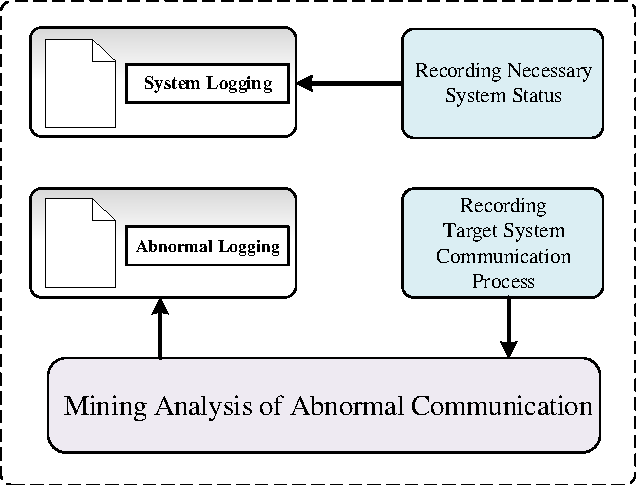
\includegraphics[width=3.2in]{FIGURE_LV/FigCollectingLogs.pdf}
	\caption{Procedure of collecting logs}
	\label{FigCollectingLogs}
\end{figure}

\begin{figure*}[htbp] 		 %  插入双栏图片
	\centering
	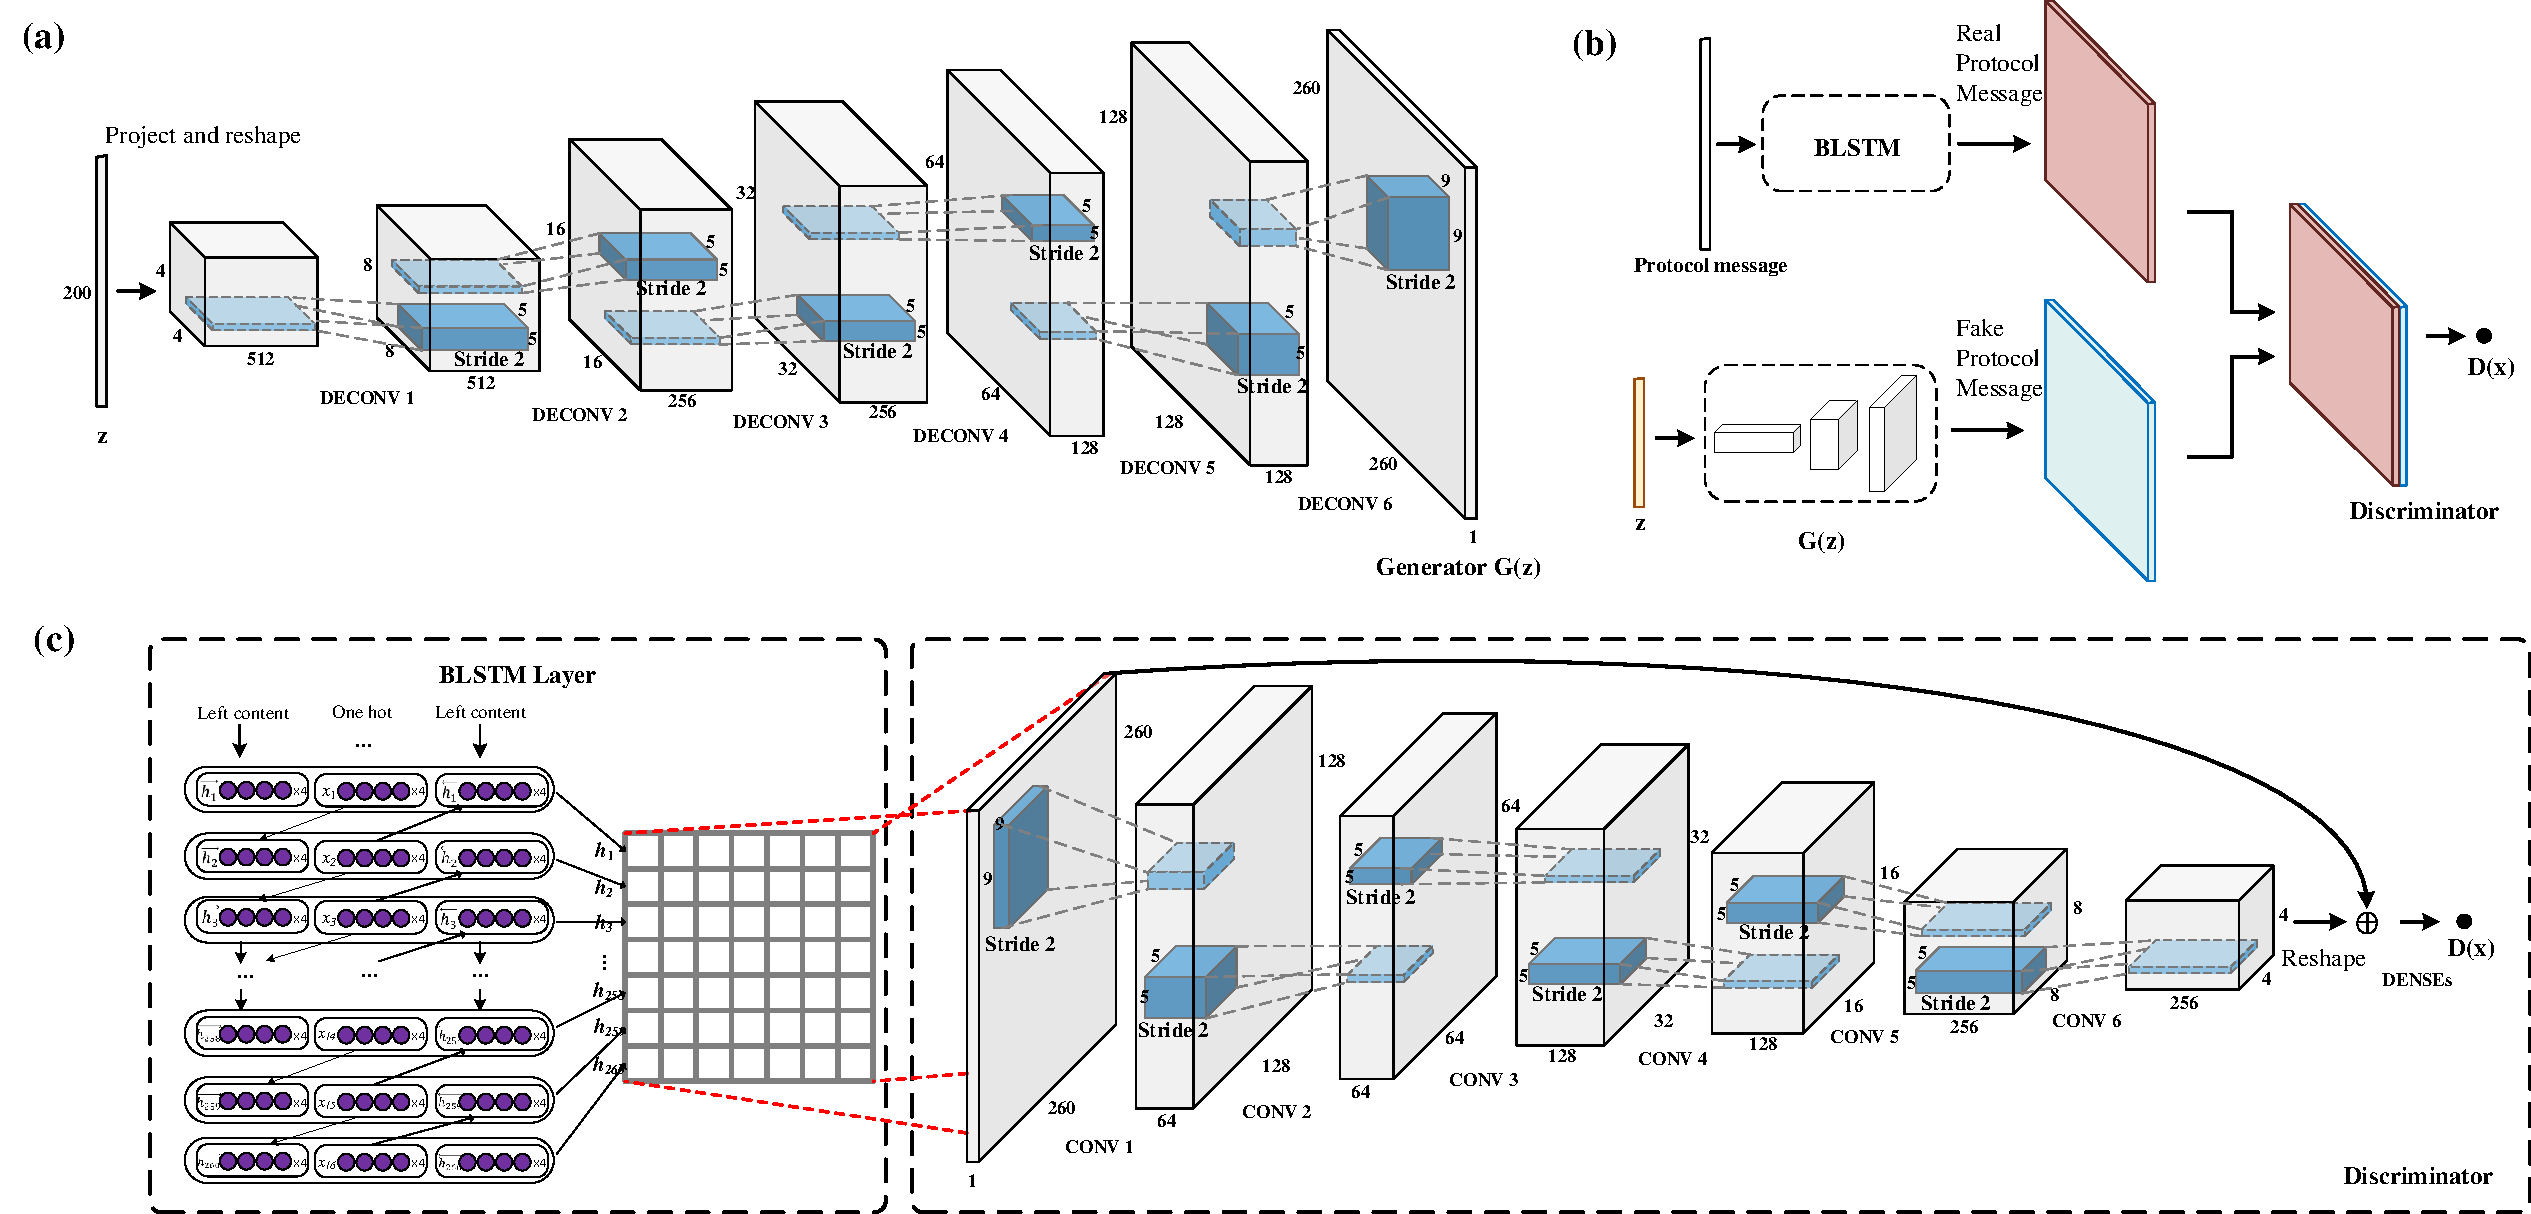
\includegraphics[width=7in]{FIGURE_LV/FigModelArchitecture.pdf}
	\caption{The architecture of DCGAN: (a) generator network, (b) architecture of DCGAN, (c) and discriminator network. The first part of (c) is a BLSTM2DCNN for the 260 byte input sequence, one hot have size 16, word embedding have size 260 and BLSTM has 260 hidden units. }
	\label{FigModelArchitecture}
\end{figure*} 